\section{Second Member - Marcus}
\subsection{Comments about the module}
The module has been quite good so far in providing me with an insight to the process of software engineering although I have felt that sometimes there are examples that aren't always clear. Also a couple of the assessed labs have felt particularly rushed and short on time.

\subsection{Selfie with Max}

\begin{figure}[h]
\caption{Selfie with Max}
\centering
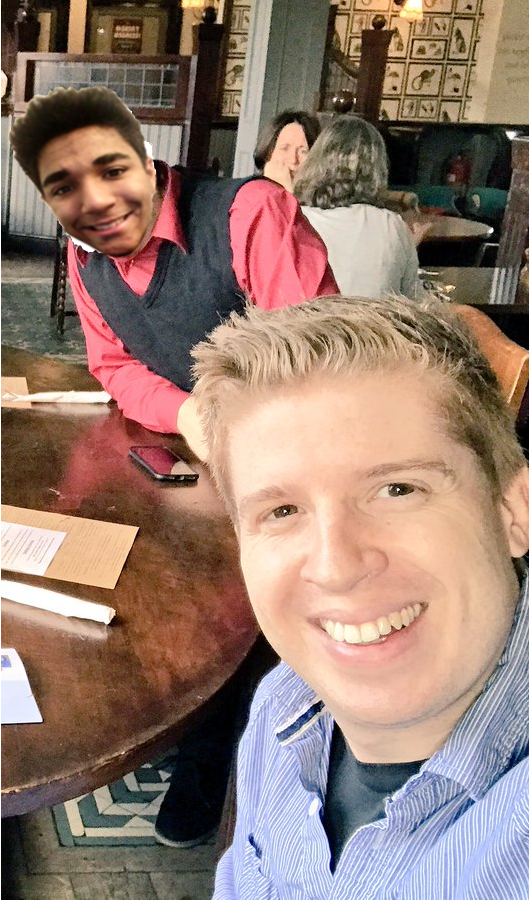
\includegraphics[width=0.5\textwidth]{editedmarcusmaxselfie.png}
\label{fig:selfie}
\end{figure}

My selfie with Max is in  Figure~\ref{fig:selfie}. (I have the best photo-editing skills ever...)

\subsection{What I have learned in this module}
So far in this module I have learnt how to analyse a given textual scenario in order to identify the stake holders, actors and use cases involved so that I can model them. I've also learnt the fundamentals for requirements engineering which is important for establishing what exactly needs to be built to minimise costs at a later date.

I've learnt some of the techniques used to investigate the systems currently in place such as focus groups, interviews and observations as well as their individual strengths and weaknesses so that I can more effectively understand systems and what individual use cases may exist within them.

Along with investigating the current systems comes the process of modelling the data gathered so that it can be more easily understood. Within this module I've come to understand the uses of different diagrams such as Use Case Diagrams, Sequence Diagrams and Activity Diagrams to model said data but also the systems to be implemented. This can be very useful later on such as using a sequence diagram to help implement a complex system that involves a lot of communication between actors and systems. I've come to understand the relationship between the diagrams and the initial analysis of the scenario and how it can make producing the models easier.

During this module I've also learnt about the key differences between the user requirements and the actual system specifications and how they are linked. I now know how to produce more structured specifications and when to use tables such as specifying exact conditions and calculations.

More recently I've been learnt about LaTeX which is a piece of software that provides are more programming-oriented way of producing a document while not having to worry about the layout allowing me to easily produce neater looking documents. I've been re-introduced to git as I had some prior experience using it but the module has provided me with a better understanding as to how the version control works in terms of saving the changes made rather than a copy of the whole file.

